% --------------------------------------------------------------------

\chapter[Cosmology]{Keeping It Even: Accurate Cosmological Measurements on the Largest Scales}
\def\chpname{cosmo}\label{chp:\chpname}

\credit{egawiser},
{\it Peter Kurczynski},
\credit{drphilmarshall},
\credit{ohadshemmer},
\credit{tanguita}
{\it and others to follow}

% --------------------------------------------------------------------

\section{Introduction}
\label{sec:\chpname:intro}

% Introduce, with a very broad brush, this chapter's science projects,
% and why it makes sense for them to be considered together.

Cosmology is one of the key science themes for which LSST was designed. Our goal is to measure cosmological parameters, such as the equation of state of dark energy, or departures from General Relativity, with sufficient accuracy to distinguish one model from another, and hence drive our theoretical understanding of how the universe works, as a whole. To do this will necessarily involve a variety of different measurements, that can act as cross-checks of each other, and break parameter degeneracies in any single one.

The  Dark Energy Science Collaboration (DESC) has identified five
different cosmological probes enabled by the LSST: weak lensing (WL),
large scale structure (LSS), type Ia supernovae (SN), strong lensing
(SL), and clusters of galaxies (CL). In all cases, the primary concern
is residual systematic error: the shapes and photometric redshifts of
galaxies, and the properties of supernova and lensed quasar light
curves, will all need to be measured with extraordinary accuracy in order for LSST's high statistical power to be properly harnessed. This accuracy will come from the abundance and heterogeneity of the individual measurements made, and the degree to which they can be modeled and understood. This latter point implies a need for uniformity in the survey, which enables powerful simplifying assumptions to be made when calibrating on the largest, cosmologically most important scales. The need for heterogeneity also implies  uniformity, in the sense that the nuisance parameters that describe the systematic effects need to be sampled over as wide a range as possible (examples include the need to sample a wide range of roll angles to minimize shape error, and observing conditions to understand photometric errors due to the changing atmosphere).

In this chapter we look at some of the key measurements planned by the Dark Energy Science Collaboration, and how they depend on the Observing Strategy.

% Anticipate the results of the chapter: summarize the results of a
% number of investigative sections, where there will be one on each
% science case.

%---------------------------------------------------------------------

% ====================================================================
%+
% SECTION NAME:
%    dithering.tex
%
% CHAPTER:
%    cosmology.tex
%
% ELEVATOR PITCH:
%    Large Scale Structure, Weak Lensing, and Clusters all require
% survey uniformity in the static 10-year survey.  A key contributor to 
%this is the pattern of dithers adopted.  
%
% COMMENTS:
%
%
% BUGS:
%
%
% AUTHORS:
%   Eric Gawiser (@egawiser)
%-
% ====================================================================
\clearpage
\section{Large Scale Structure:  Testing Dithering Patterns and Timescales to Improve Survey Uniformity}
\def\secname{dithering}\label{sec:\secname}

\noindent{\it Humna Awan, Eric Gawiser, Peter Kurczynski, Lynne Jones} % (Writing team)

% This individual section will need to describe the particular
% discoveries and measurements that are being targeted in this section's
% science case. It will be helpful to think of a ``science case" as a
% ``science project" that the authors {\it actually plan to do}. Then,
% the sections can follow the tried and tested format of an observing
% proposal: a brief description of the investigation, with references,
% followed by a technical feasibility piece. This latter part will need
% to be quantified using the MAF framework, via a set of metrics that
% need to be computed for any given observing strategy to quantify its
% impact on the described science case. Ideally, these metrics would be
% combined in a well-motivated figure of merit. The section can conclude
% with a discussion of any risks that have been identified, and how
% these could be mitigated.

% A short preamble goes here. What's the context for this science
% project? Where does it fit in the big picture?

Three of the key cosmology probes available with LSST represent ``static science'' insensitive to time-domain concerns.  These are Weak Lensing, Large-Scale Structure, and Galaxy Clusters.  Nonetheless, due to the need to track and correct for the survey ``window function'' in all of these probes, cosmology with LSST will benefit greatly from achieving survey depth as uniform as possible over the WFD area.  OpSim tiles the sky in hexagons inscribed within the nearly-circular LSST field-of-view.  It has been shown in \citet{CarrollEtal2014} that the default LSST survey strategy implemented in OpSim runs leads to a strongly non-uniform ``honeycomb'' pattern due to overlapping regions on the edges of these hexagons receiving double the observing time.  A pattern of large dithers proves sufficient to greatly reduce these overlaps, leading to an increase in median survey depth in each filter of 0.08 magnitudes.  

In this section, we report results from an investigation by Awan et al. (in preparation) of several geometrical patterns for dithers performed on timescales varying from once per observing season to once per night to every visit.  

\todo{EG}{Flesh out WL, LSS, and Clusters dependence on survey uniformity to make this section more clearly science-driven.}  

% --------------------------------------------------------------------

\subsection{Dithering Patterns and Timescales}
\label{sec:\secname:strategies}


% --------------------------------------------------------------------

\subsection{Metrics}
\label{sec:\secname:metrics}

% Quantifying the response via MAF metrics: definition of the metrics,
% and any derived overall figure of merit.

Our primary metric is total uncertainty in the derived window function over relevant angular scales, modeled via variations in the angular power spectrum of fake galaxy fluctuations between $gri$ bands.  
Intermediate metrics include the number of galaxies in 
each pixel, fluctuations in this number, total power in the angular power spectrum of a skymap of those fluctuations, and residual power that angular power spectrum after subtracting a smooth fit to it.  



% --------------------------------------------------------------------

\subsection{OpSim Analysis}
\label{sec:\secname:analysis}

% OpSim analysis: how good would the default observing strategy be, at
% the time of writing for this science project?

In this section we present our ongoing \OpSim / MAF
analysis, as we try to
answer the question ``what dithering strategies produce acceptable variations in survey uniformity, and which appears optimal?''

%We used the
%\simsMAFcontrib{SeasonStacker}{mafContrib/seasonStacker.py} to work
%with seasons.

%We used \texttt{ops2\_1075} for most of our tests, but we need to now
%re-run on \opsimdbref{db:enigma}, and others from \autoref{chp:cadence2015}.


%\citeauthor{LiaoEtal2015}). These sky maps show that, over the main

%\autoref{tab:lenstimedelays:results} shows the global (i.e. al-sky)


%--------------------------------------------------------------------

\subsection{Results}
\label{sec:\secname:results}


\todo{EG}{Improve figures to originals rather than screen-captures.}


%%%%%%%%%%%%%%%%%%%%%%%%%%%%%%%%%
\begin{figure}[tbh!]
\vskip -0.1in
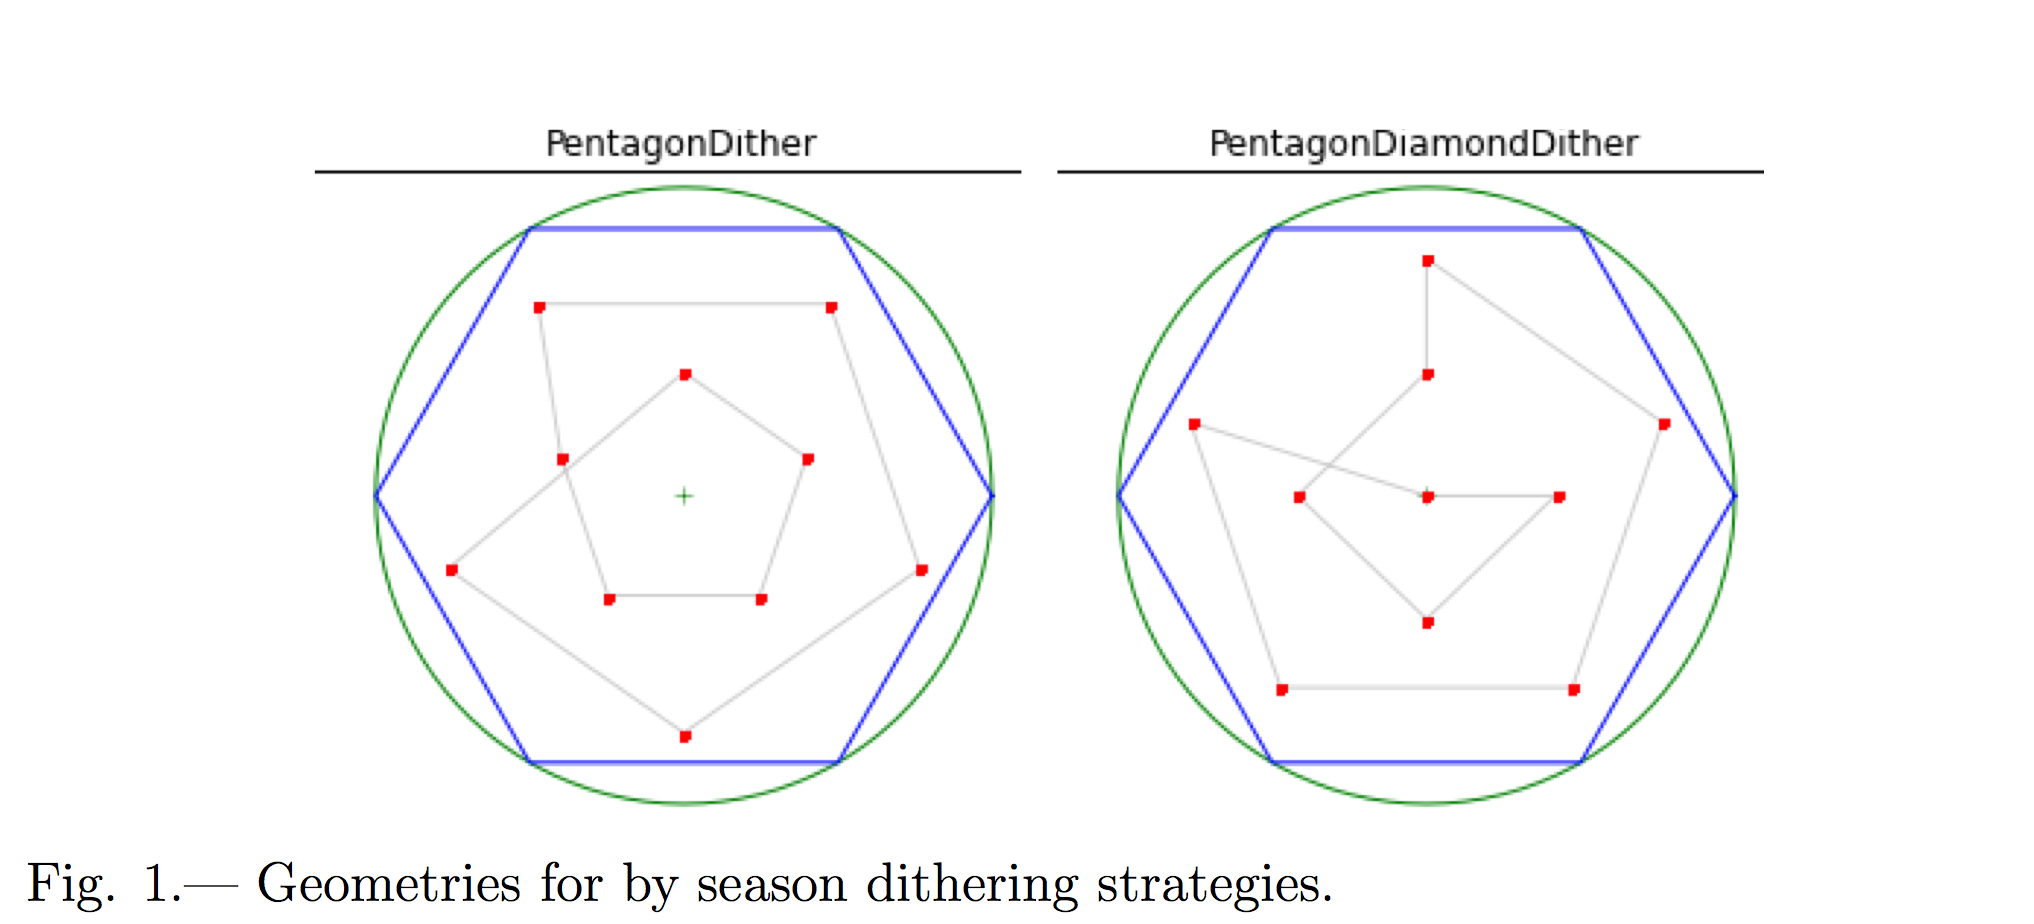
\includegraphics[angle=0,width=0.99\hsize:,clip]{figs/awan_fig1.png}
%\vskip -1.3in
\caption{}
\label{fig:seasonal_dithers}
\end{figure}
%%%%%%%%%%%%%%%%%%%%%%%%%%%%%%%%%

%%%%%%%%%%%%%%%%%%%%%%%%%%%%%%%%%
\begin{figure}[tbh!]
\vskip -0.1in
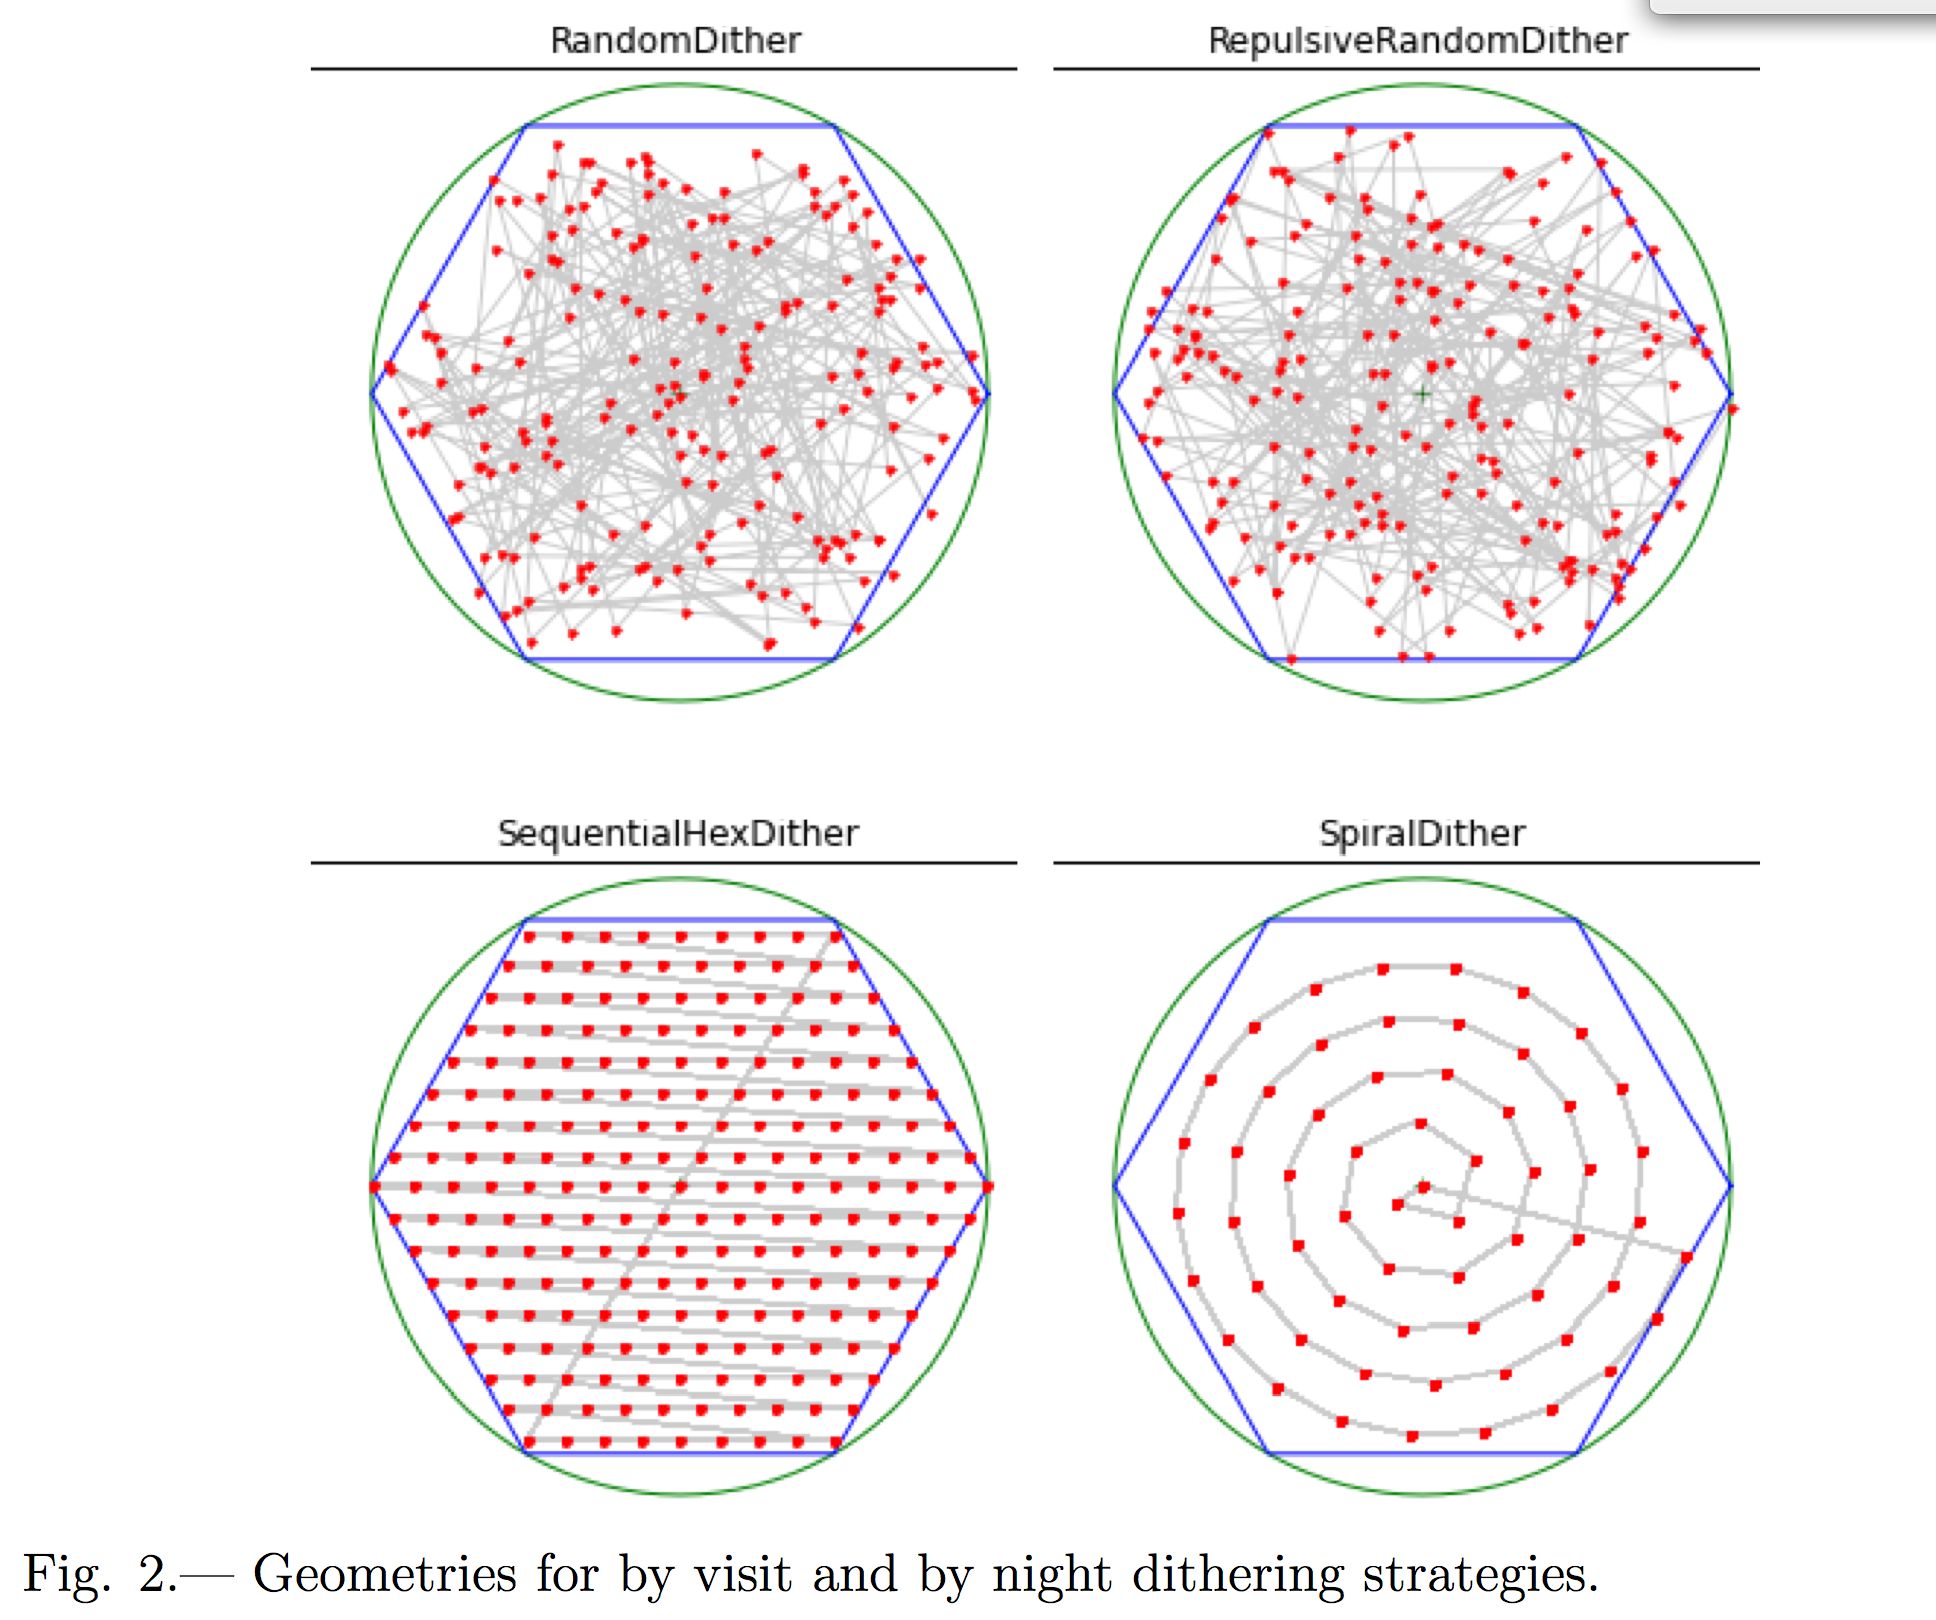
\includegraphics[angle=0,width=0.99\hsize:,clip]{figs/awan_fig2.png}
%\vskip -1.3in
\caption{}
\label{fig:nightly_dithers}
\end{figure}
%%%%%%%%%%%%%%%%%%%%%%%%%%%%%%%%%

%%%%%%%%%%%%%%%%%%%%%%%%%%%%%%%%%
\begin{figure}[tbh!]
\vskip -0.1in
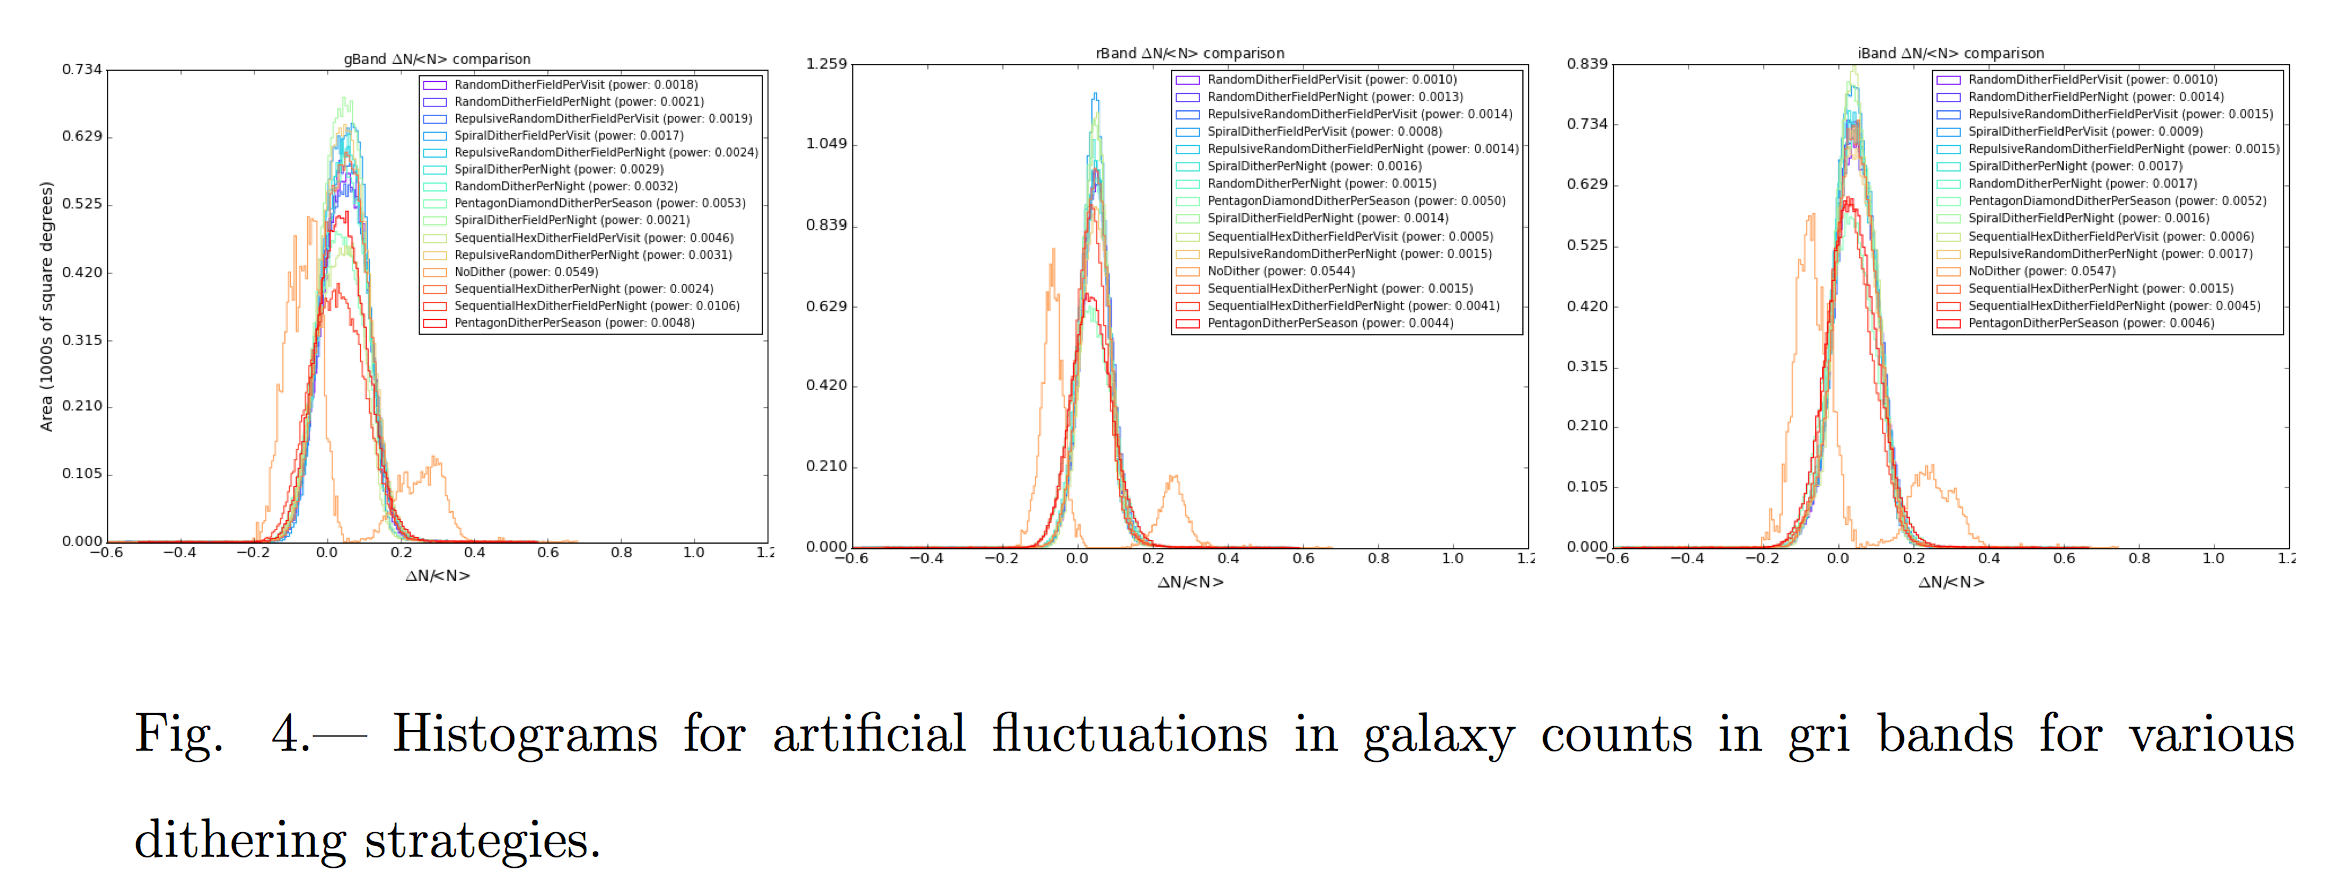
\includegraphics[angle=0,width=0.99\hsize:,clip]{figs/awan_fig4.png}
%\vskip -1.3in
\caption{}
\label{fig:dithering_histograms}
\end{figure}
%%%%%%%%%%%%%%%%%%%%%%%%%%%%%%%%%

%%%%%%%%%%%%%%%%%%%%%%%%%%%%%%%%%
\begin{figure}[tbh!]
\vskip -0.1in
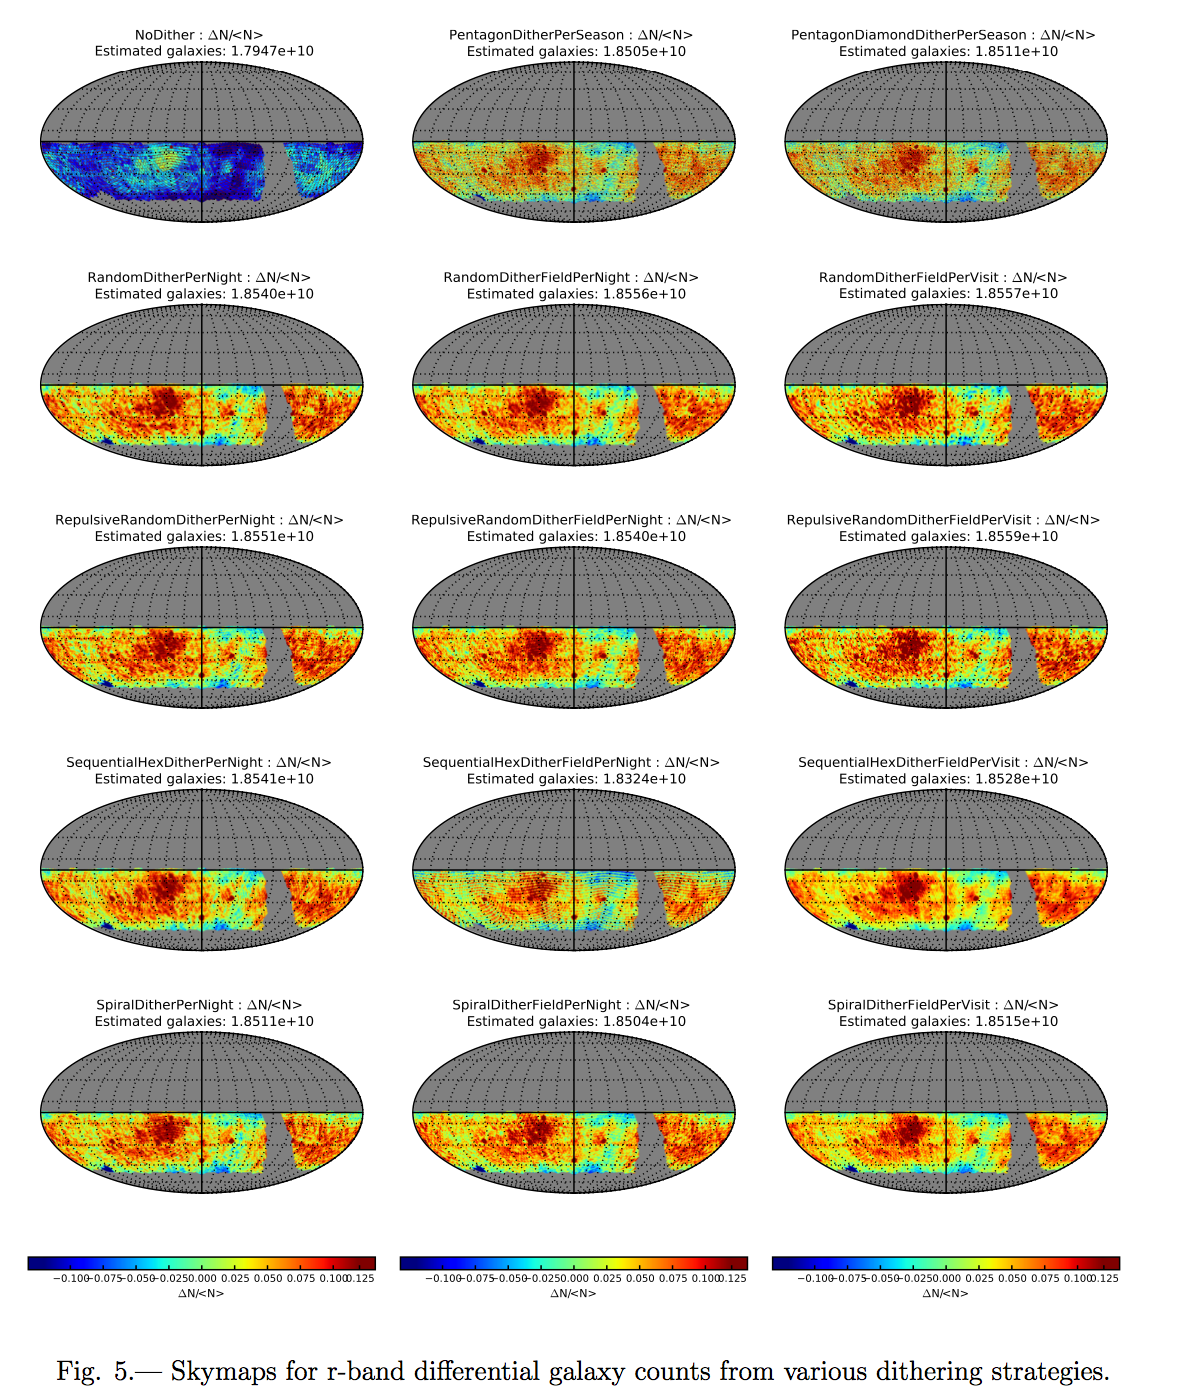
\includegraphics[angle=0,width=0.99\hsize:,clip]{figs/awan_fig5.png}
%\vskip -1.3in
\caption{}
\label{fig:dithering_skymaps}
\end{figure}
%%%%%%%%%%%%%%%%%%%%%%%%%%%%%%%%%

%%%%%%%%%%%%%%%%%%%%%%%%%%%%%%%%%
\begin{figure}[tbh!]
\vskip -0.1in
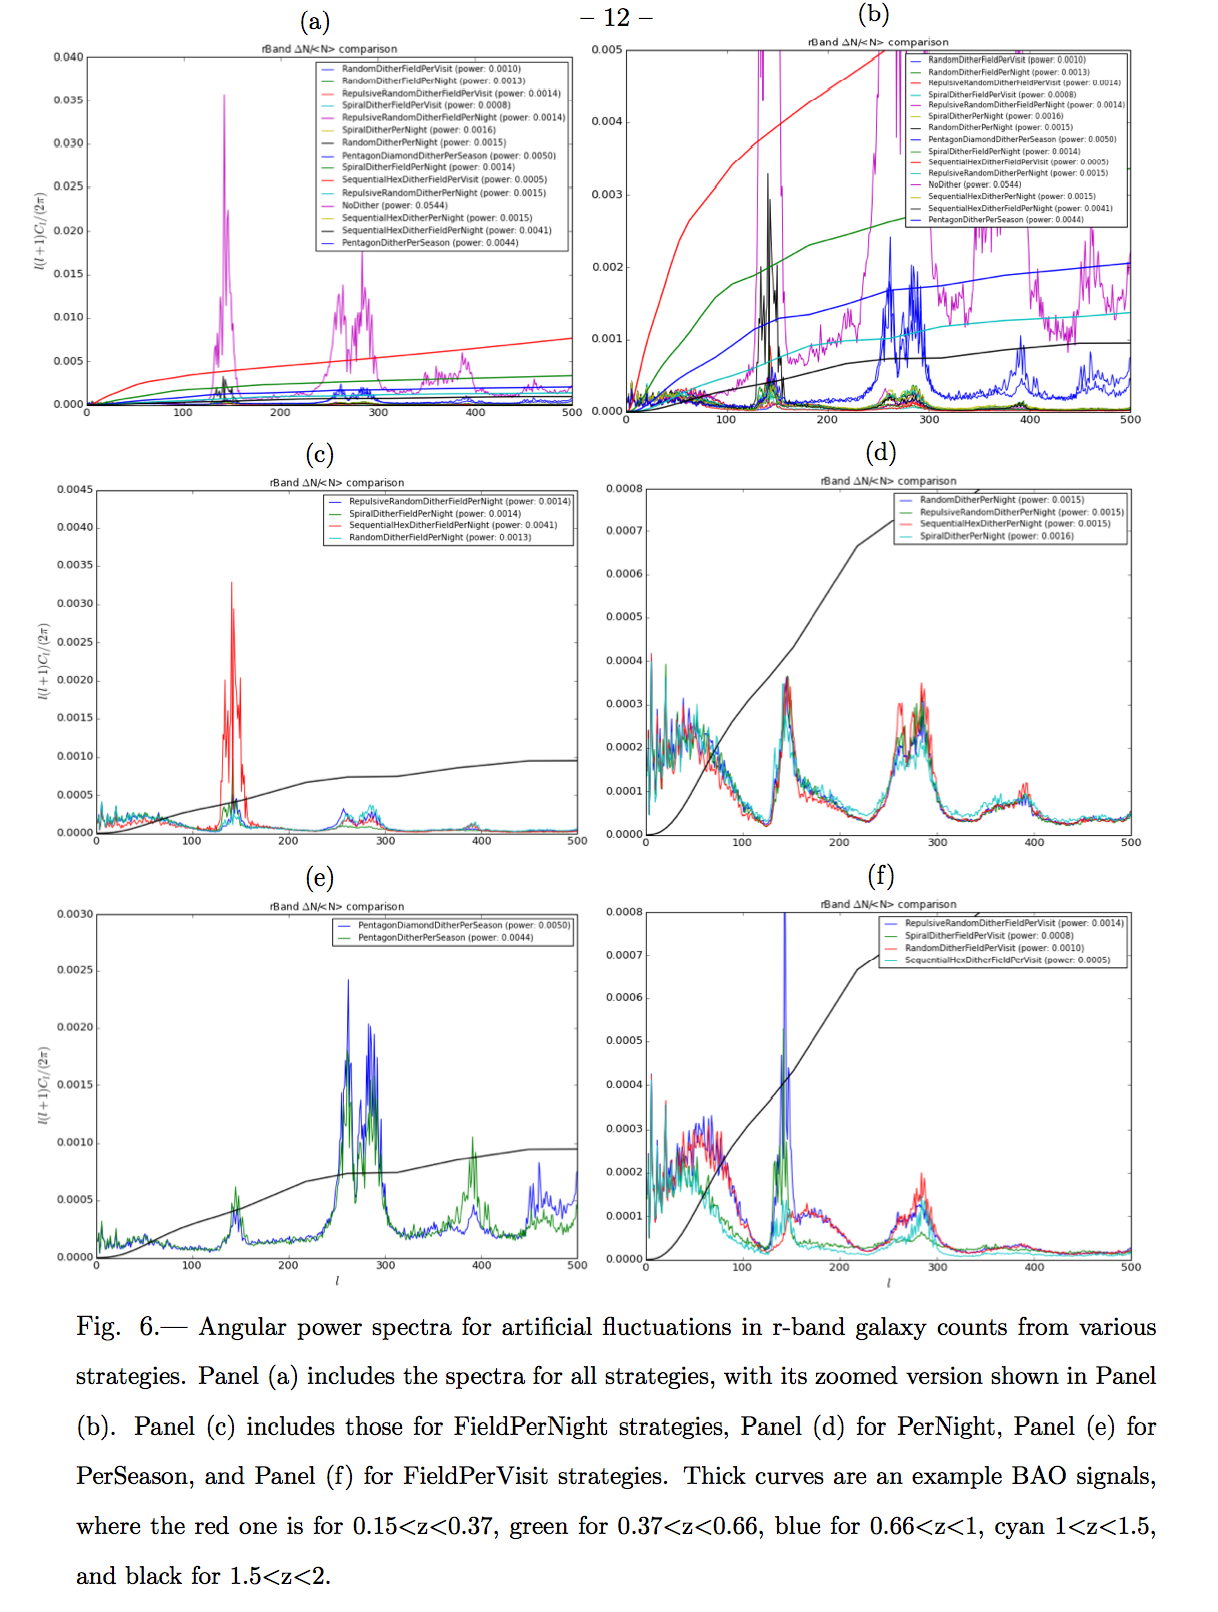
\includegraphics[angle=0,width=0.99\hsize:,clip]{figs/awan_fig6.png}
%\vskip -1.3in
\caption{}
\label{fig:dithering_power_spectra}
\end{figure}
%%%%%%%%%%%%%%%%%%%%%%%%%%%%%%%%%




%%%%%%%%%%%%%%%%%%%%%%%%%%%%%%%%%%%%
%\begin{figure*}[!ht]
%  \capstart
%  \begin{minipage}[b]{\linewidth}
%    \begin{minipage}[b]{0.32\linewidth}
%      \centering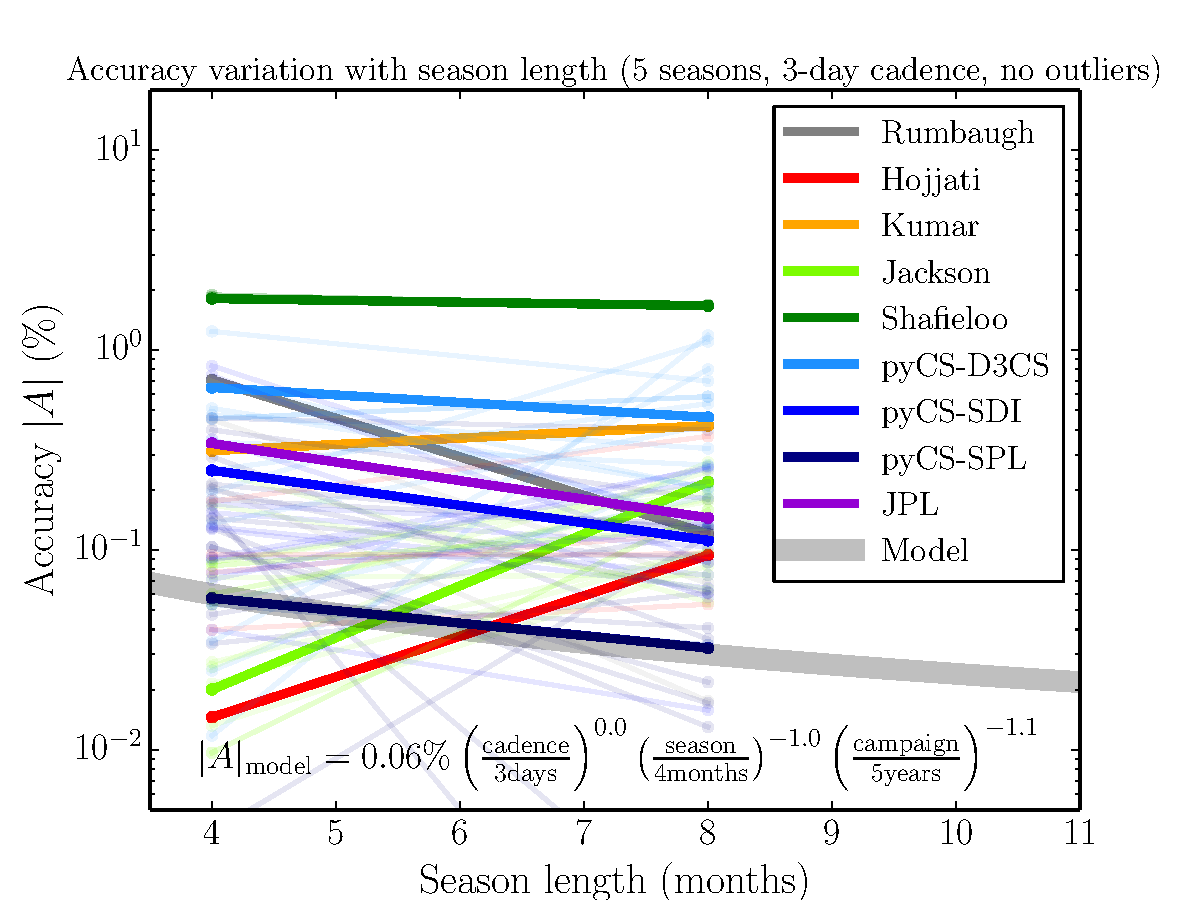
\includegraphics[width=\linewidth]{figs/Accuracy_season_nca.pdf}
%    \end{minipage} \hfill
%    \begin{minipage}[b]{0.32\linewidth}
%      \centering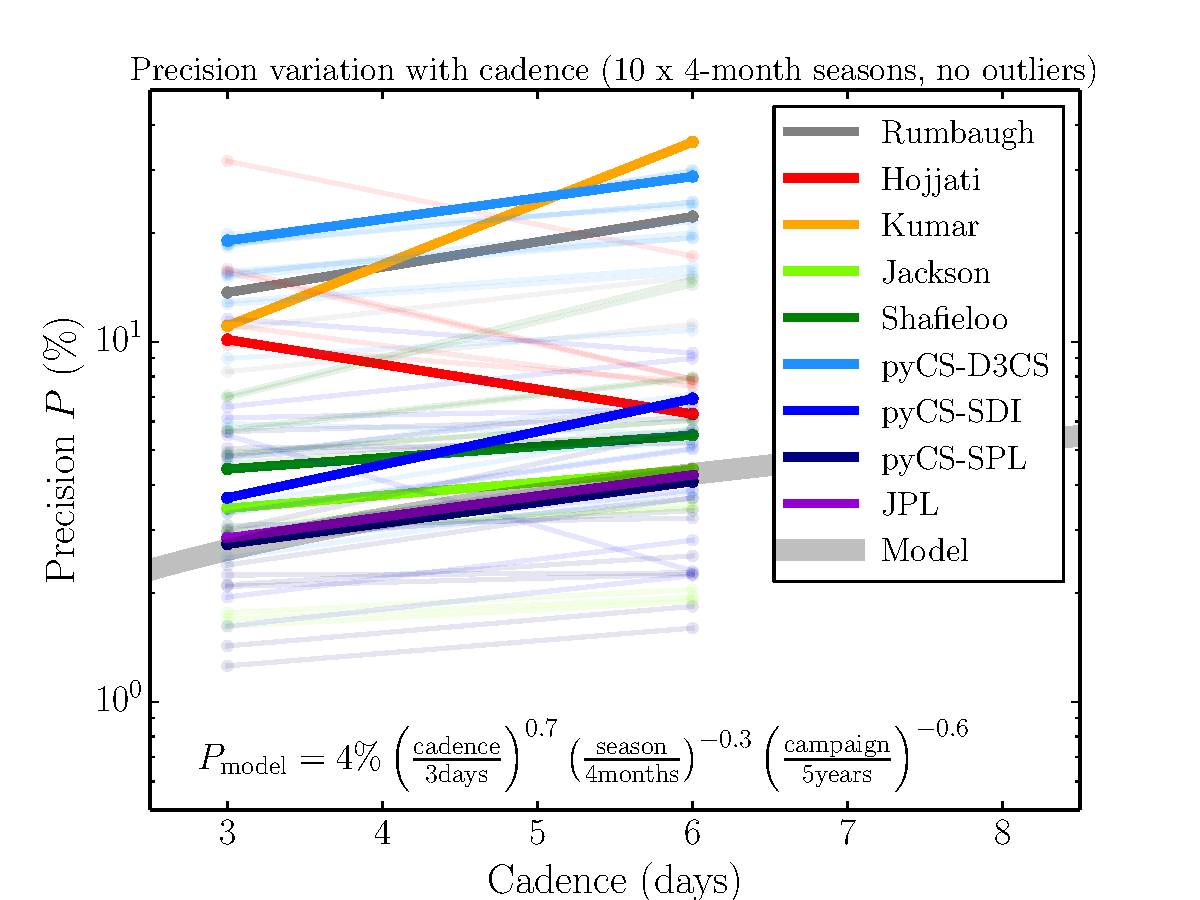
\includegraphics[width=\linewidth]{figs/Precision_cadence_nca.pdf}
%    \end{minipage} \hfill
%    \begin{minipage}[b]{0.32\linewidth}
%      \centering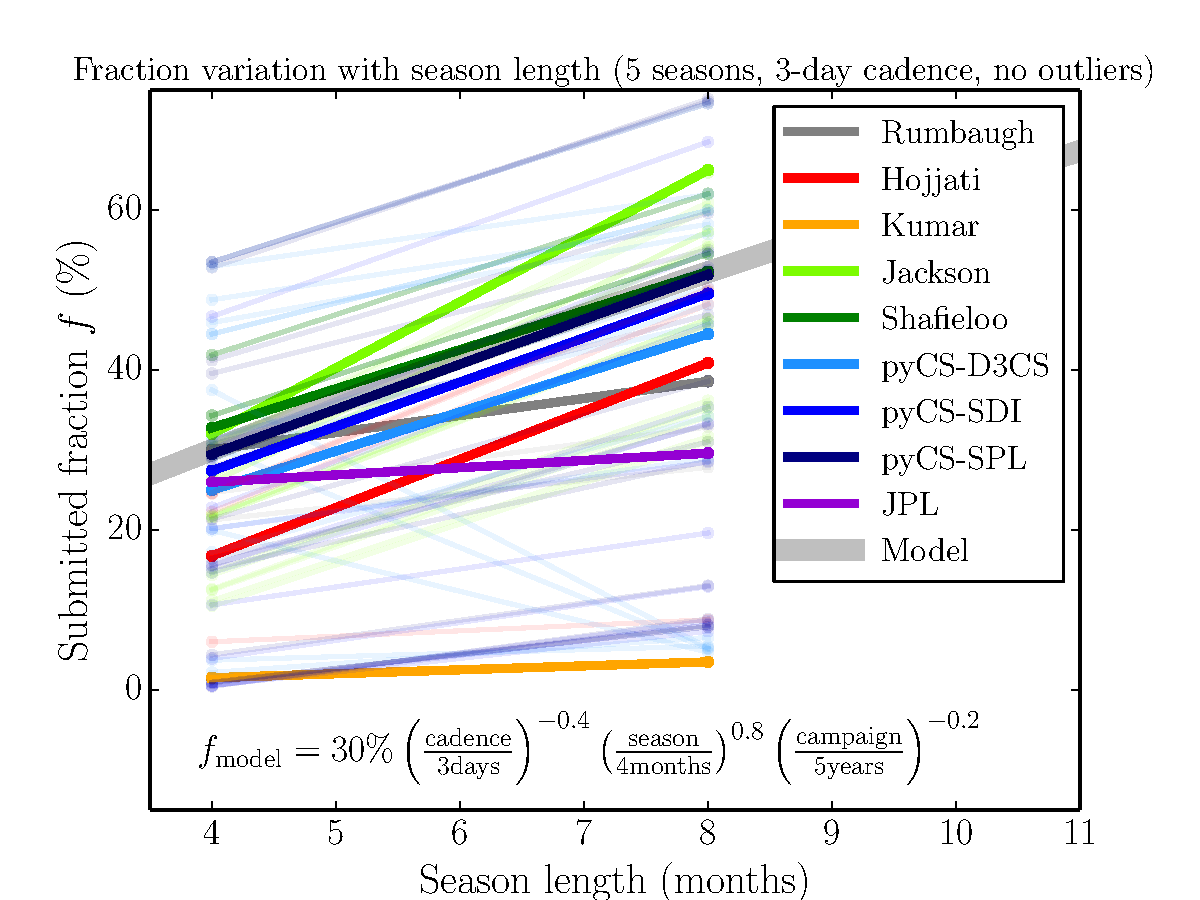
\includegraphics[width=\linewidth]{figs/Fraction_season_nca.pdf}
%    \end{minipage}
%  \end{minipage}
%\caption{Examples of changes in accuracy $A$ (left), precision $P$ (center) and success fraction $f$ (right) with schedule properties, as seen in the different TDC submissions. The gray
%approximate power law model was derived by visual inspection of the
%pyCS-SPL results; the signs of the indices were pre-determined according to our expectations. Reproduced from \citet{LiaoEtal2015}.}
%\label{fig:tdcresults}
%\end{figure*}
%%%%%%%%%%%%%%%%%%%%%%%%%%%%%%%%%%%


\todo{EG}{Input fuller results and text from Awan et al. draft.}  

%---------------------------------------------------------------------

\subsection{Discussion}
\label{sec:\secname:discussion}



\navigationbar

% ====================================================================
  

% --------------------------------------------------------------------

% ====================================================================
%+
% NAME:
%    lenstimedelays.tex
%
% ELEVATOR PITCH:
%    Lensed quasars and supernovae provide distance measurements for
%    cosmology. They are a few days to a few weeks in length. To
%    measure them well we need long campaigns (>~3 years) with high
%    night-to-night cadence (better than the standard 5 days if
%    possible, especially as combining all filters might be difficult.)
%
% COMMENTS:
%
%
% BUGS:
%
%
% AUTHORS:
%   Phil Marshall (@drphilmarshall)
%-
% ====================================================================

\section{ Strong Gravitational Lens Time Delays }
\label{sec:lenstimedelays}

\noindent{\it Phil Marshall} % (Writing team)

% This individual section will need to describe the particular
% discoveries and measurements that are being targeted in this section's
% science case. It will be helpful to think of a ``science case" as a
% ``science project" that the authors {\it actually plan to do}. Then,
% the sections can follow the tried and tested format of an observing
% proposal: a brief description of the investigation, with references,
% followed by a technical feasibility piece. This latter part will need
% to be quantified using the MAF framework, via a set of metrics that
% need to be computed for any given observing strategy to quantify its
% impact on the described science case. Ideally, these metrics would be
% combined in a well-motivated figure of merit. The section can conclude
% with a discussion of any risks that have been identified, and how
% these could be mitigated.

A short preamble goes here. What's the context for this science
project? Where does it fit in the big picture?

% --------------------------------------------------------------------

\subsection{Target measurements and discoveries}
\label{sec:lenstimedelays:targets}

Describe the discoveries and measurements you want to make.

Now, describe their response to the observing strategy. Qualitatively,
how will the science project be affected by the observing schedule and
conditions? In broad terms, how would we expect the observing strategy
to be optimized for this science?


% --------------------------------------------------------------------

\subsection{Metrics}
\label{sec:lenstimedelays:metrics}

Quantifying the response via MAF metrics: definition of the metrics,
and any derived overall figure of merit.


% --------------------------------------------------------------------

\subsection{OpSim Analysis}
\label{sec:lenstimedelays:analysis}

OpSim analysis: how good would the default observing strategy be, at
the time of writing for this science project?


% --------------------------------------------------------------------

\subsection{Discussion}
\label{sec:lenstimedelays:discussion}

Discussion: what risks have been identified? What suggestions could be
made to improve this science project's figure of merit, and mitigate
the identified risks?


% ====================================================================


% --------------------------------------------------------------------

% ====================================================================
%+
%
% SECTION NAME:
%    \secname.tex
%
% CHAPTER:
%    ???.tex
%
%
% COMMENTS:
%
%
% BUGS:
%
%
% AUTHORS:
%   Ohad Shemmer (@ohadshemmer), Timo Anguita (@tanguita), Niel Brandt, Gordon Richards, Scott Anderson(?),
%   Phil Marshall(?) (@drphilmarshall) 
%-
% ====================================================================

\section{AGN Science}
\def\secname{agn}\label{sec:\secname}

\noindent{\it Ohad Shemmer, Timo Anguita, Niel Brandt, Gordon Richards, Scott Anderson(?), Phil Marshall(?)}

% This section discusses the potential effects of the LSST observing strategy on AGN science. In short, there appears to be
% a consensus among the AGN and galaxies communities that AGN science will benefit from the most uniform cadence in
% terms of even sampling for each band and uniform sky coverage. It is also expected that any reasonable
% perturbation to the nominal LSST observing strategy will have mostly minor effects on AGN science. This section attempts
% to identify all the areas of AGN science that may be affected by the observing strategy and to point out the metrics that
% can be used to quantify any potential effect. Since the total number of metrics that must be quantified is quite large, and
% the effects are likely small in most cases, the goal of this section is to identify potential ``killers'' that may undermine
% key AGN research areas. For example, certain perturbations may reduce significantly the number of ``interesting'' AGNs,
% such as $z>6$ quasars, lensed quasars, or transient AGNs. Another example is photometric reverberation mapping
% which is one of LSST's greatest advantages for AGN research but is also very sensitive to the cadence; care must
% be taken to ensure that the observing strategy does not undermine the ability to make the best use of this method.

\subsection{AGN Selection and Census}
\label{sec:\secname:selection}

\noindent About $10^7 - 10^8$ AGNs will be selected in the main LSST survey using a combination of criteria, split
broadly into four categories: colors, astrometry, variability, and multiwavelength matching with other surveys.
The LSST observing strategy will affect mostly the first three of these categories.

{\bf Colors:}~The LSST observing strategy will determine the depth in each band, as a function of position on the sky, and will thus affect
the color selection of AGNs. This will eventually determine the AGN $L-z$ distribution and, in particular, may affect the identification
of quasars at $z\gtsim 6$ if, for example, $Y$-band exposures will not be sufficiently deep.

{\bf Variability:} AGNs can be effectively distinguished from (variable) stars, and from quiescent galaxies, by exhibiting certain characteristic variability patterns (e.g., Butler \& Bloom 2011). Non-uniform sampling may ``contaminate'' the variability signal of AGN candidates.

{\bf Astrometry:} AGNs will be selected among sources having zero proper motion, within the uncertainties. The LSST cadence
may affect the level of this uncertainty in each band, and may therefore affect the ability to identify (mostly fainter) AGNs.
%
Differential chromatic refraction (DCR), making use of the astrometric offset a source with emission lines has with respect to
a source with a featureless power-law spectrum, can help in the selection of AGNs and in confirming their photometric redshifts (Kaczmarczik~et~al.~2009). The DCR effect is more pronounced at higher airmasses. AGN selection and photometric redshift confirmation may be affected since the LSST cadence will affect the airmass distribution, in each band, for each AGN candidate.

\subsection{AGN Clustering}
\label{sec:\secname:clustering}

\noindent Measurements of the spatial clustering of AGNs with respect to those of quiescent galaxies can provide clues as to how galaxies
form inside their dark-matter halos and what causes the growth of their supermassive black holes (SMBHs). The impressive inventory 
of LSST AGNs will enable the clustering, and thus the host galaxy halo mass, to be determined over the widest range ranges of cosmic
epoch and accretion power.
%
The LSST cadence will not only affect the overall AGN census and its $L-z$ distribution, but also the
depth in each band as a function of sky position that can directly affect the clustering signal.

\subsection{AGNs and the Time Domain}
\label{sec:\secname:time}

{\bf AGN Variability:} A variety of AGN variability studies will be enabled by LSST. These are intended to probe the physical properties of the unresolved inner regions of the central engine. Relations will be sought between variability amplitude and timescale vs. $L$, $z$, $\lambda_{\rm eff}$, color, multiwavelength and spectroscopic properties, if available. The LSST sampling is expected to provide high-quality power spectral density functions for a large number of AGNs; these can be used to constrain the SMBH mass and accretion rate/mode. Furthermore, LSST AGNs exhibiting excess variability over that expected from their luminosities will be further scrutinized as candidates for lensed systems having unresolved images with the excess (extrinsic) variability being attributed mainly to microlensing.

Photometric reverberation mapping (PRM), measuring the time-delayed response of either the flux of the broad emission line region (BELR) lines to the flux of the AGN continuum or between the continuum flux in one (longer wavelength) band to the continuum flux in another (band with shorter wavelength), will be one of the cornerstones of AGN research in the LSST era
(e.g., Chelouche 2013; Chelouche \& Zucker 2013; Chelouche~et~al.~2014). For example, LSST is expected to deliver BELR line-continuum time delays in $\sim10^5-10^6$ sources, which is unprecedented when compared to $\sim50-100$ such measurements conducted via the traditional, yet much more expensive (per source) spectroscopic method. Sources in the deep-drilling fields (DDFs) will benefit from the highest quality PRM
time-delay measurements given the factor of $\sim10$ denser sampling. The PRM measurements will probe the size and structure of the accretion disk and BELR, in a statistical sense, and may provide improved SMBH mass estimates for sources that have at least single-epoch spectra.

The PRM method is very sensitive to the sampling in each band, therefore the ability to derive reliable time delays can be affected significantly
by the LSST cadence. The best results will be obtained by having the most uniform sampling equally for each band. Additionally, there is
a trade-off between the number of DDFs and the number of time delays that PRM can obtain (Chelouche~et~al.~2014). For example,
an increase in the number of DDFs, with similarly dense sampling in each field, can yield a proportionately larger number of high-quality time delays,
down to lower luminosities, but at the expense of far fewer time delays (of relatively high luminosity sources) in the main survey.

{\bf Time Delays in Gravitationally Lensed Quasars:} This aspect is discussed in detail in the lenstimedelays.tex section.

{\bf AGN Size and Structure with Microlensing:} Microlensing due to stars projected on top of individual lensed quasar images produce additional magnification. Using the fact that the Einstein radii of stars in lensing galaxies closely match the scales of different emission regions in high-redshift AGNs (micro-arcseconds), analyzing microlensing induced flux variations statistically on individual systems allows us to measure ``sizes'' of AGN regions.
%
Assuming a thermal profile for accretion disks, sizes in different emission wavelengths will be probed and as such, constraints on the slope of this thermal profile. Given the sheer number of lensed systems that LSST is expected to discover ($\sim8000$), this will allow us to stack systems for better constraints and hopefully determine the evolution of the size and profile. Due to the typical relative velocities of lenses, microlenses, observers (Earth) and source AGN, the microlensing variation timescales are between months to a few decades.

The quasar microlensing optical depth is $\sim1$, so every lensed quasar should be affected by microlensing at any given point in time. However, measurable variability can occur on longer timescales. Mosquera~et~al.~(2011) did a study using all known lensed quasars. They found the median timescale between high magnification events (Einstein crossing time scales) in the observed $I$-band is of the order of $\sim20$~yr (with a distribution between 10 and 40~yr). However, the source crossing time (duration of a high magnification event) is $\sim7.3$~months (with a distribution tail up to 3~yr). This basically means that out of all the lensed quasar {\em images} (microlensing between images is completely uncorrelated) about half of them will be quiescent during the 10~yr baseline of LSST. However, since the typical number of lensed images is either two or four, it means that, statistically, in every system, one (for doubles) or two (for quads) high magnification events should be observed in 10~yr of LSST monitoring.

Note that, the important cadence parameter is the source crossing time, as it is the length of the event to be as uniformly sampled as possible. The 7.3 months crossing time is the median for the observed $i$-band, but this time would be significantly shorter for bluer bands: for a thermal profile with slope $\alpha: R_\lambda \propto \lambda^\alpha$ implies source crossing time $t_{\rm s} \propto \lambda^{1/\alpha} \rightarrow t_u=t_i \times (\lambda_{\rm u} / \lambda_{\rm i})^{1/\alpha}$. For a Shakura-Sunyaev slope of $\alpha=0.75$ this would correspond to $7.3 \times (3600/8140)^{4/3}$ months $\approx 2.5$ months in the $u$-band.

In terms of the cadence, at least three evenly sampled data points per band within 2 to 3 months would be preferred to be able to map the constraining high magnification event(?). Hopefully uniformly spaced. Very tight cadence (e.g., DDFs) would increase the constraints significantly. However, since lensed quasars are not that common, this smaller area would mean only a few ($\sim80$?) suitable systems monitored in the DDFs.
%
Regarding the season length, the ``months'' timescale of high magnification events very likely means that we can/will miss high magnification events in the season gaps, at least in the bluer bands.
%
Killer: observations spread on timescales larger than 3 months(??). This would likely miss the high magnification events. In those cases we could perhaps consider close consecutive photometric bands as equivalent accretion disk regions, however this would mean weaker constraints on the thermal profile.
%
Important Note: all this science needs to be done on lensed quasars with measured or very short time delays to remove the intrinsic variability signal, which might significantly reduce the sample.

{\bf Microlensing Aided Reverberation Mapping:} Given that microlensing mostly affects continuum emission rather than BELR line emission, microlensing may enable disentangling the BELR line $+$ continuum emission in single photometric bands, allowing the use of single broad band PRM measurements (Sluse \& Tewes 2014). As with the two-band PRM method discussed above, the denser (and the longer) the sampling, the more accurate are the constraints that can be obtained for the time delays.

{\bf Transient AGN and TDEs:} This aspect is discussed in detail in the variablesandtransients.tex section(?)

% --------------------------------------------------------------------

\subsection{Metrics}
\label{sec:\secname:metrics}

% Quantifying the main impacts on AGN science via MAF metrics, including the effects
% of additional cadence facto,rs such as the number of DDFs
% and MC fields, or different dithering patterns,: definition of the metrics,
% and any derived overall figure of merit.

% --------------------------------------------------------------------

\subsection{Discussion}
\label{sec:\secname:discussion}

% Discussion: what risks have been identified? What suggestions could be
% made to improve the figures of merit, and mitigate the identified risks?
% What ``tweaks'', if any, can be proposed to the nominal LSST observing strategy
% in order to help achieve key AGN science goals?

\navigationbar


% --------------------------------------------------------------------

% ====================================================================
%+
% SECTION:
%    supernovacosmology.tex
%
% CHAPTER:
%    cosmology.tex
%
% ELEVATOR PITCH:
%    SNIa cosmology, approach to evaluating dependence of science on cadence
%
% COMMENTS:
%
%
% BUGS:
%
%
% AUTHORS:
%    Phil Marshall (@drphilmarshall)  - put your name and GitHub username here!
%-
% ====================================================================

\section{Supernova Cosmology and Physics}
\def\secname{supernovae}\label{sec:\secname}
% \label{sec:cosmology, supernovae, classification, lenstimedelays, deepdrillingfields }

\noindent{\it Jeonghee Rho, Michelle Lochner, Rahul Biswas} % (Writing team)

% This individual section will need to describe the particular
% discoveries and measurements that are being targeted in this section's
% science case. It will be helpful to think of a ``science case" as a
% ``science project" that the authors {\it actually plan to do}. Then,
% the sections can follow the tried and tested format of an observing
% proposal: a brief description of the investigation, with references,
% followed by a technical feasibility piece. This latter part will need
% to be quantified using the MAF framework, via a set of metrics that
% need to be computed for any given observing strategy to quantify its
% impact on the described science case. Ideally, these metrics would be
% combined in a well-motivated figure of merit. The section can conclude
% with a discussion of any risks that have been identified, and how
% these could be mitigated.

This section is concerned with the detection and characterization of supernovae (SNe)
over time with LSST and their various scientific applications.
The most important
application is the use of supernovae type Ia (SNIa) and potentially some core-collapse SN (like type IIP) to trace the recent expansion history of the universe,
and confront models of the physics driving the late time accelerated expansion
of the universe. 

This objective of SN cosmology follows (at least for SNIa) results from several
highly successful surveys; improvement in knowledge of SN cosmology could come from
substantially larger numbers of well-characterized SNe and potentially
useful redshift distributions of such detected SNe. In this sense, this
goal is not directly tied to the unprecedentedly large survey area of LSST.  
However, we shall argue that in practice, even this
goal would benefit from the spatial scale offered by the Wide Fast Deep
(WFD) component of the LSST survey. 

On the other hand, the WFD component of the LSST survey is potentially the 
first single survey to scan for SNe across the very large area of the
entire Southern sky.  SNe that are detected and well characterized by LSST will
probe the isotropy of the universe.  Peculiar velocities of 
SNe will probe the growth of structure.  In addition, this large sample
will enable further
sharpening of our understanding of the properties of the supernova population 
of different types. 
This last point is extremely important for SN cosmology goals:  The success of SNIa cosmology has always been based on the empirical model that intrinsic peak brightnesses are related to the certain observable characteristics of SNe. 
%While the spatial locations of the SNe are not important
The 
WFD has the potential to dramatically increase the size of the sample 
available to train such an empirical model, as well understand the probability of deviations and scatter from this model. Aside from issues like calibration 
which need to be addressed differently, a larger sample of such well measured SNe is probably the only way to address `systematics' due to deviations from the empirical
model. The anticipated sample can be thought of as consisting of two 
components:  the low-redshift sample which is more likely to be complete, and the higher-redshift sample that will be able to constrain evolution. 
% --------------------------------------------------------------------

\subsection{Target measurements and discoveries}
\label{sec:keyword:targets}

% Describe the discoveries and measurements you want to make.

SNe of different types are visible over time scales of about a few 
weeks (e.g., type Ia) to nearly a year (type IIP).  During the full ten-year
 survey, LSST will scan the entire southern sky repeatedly
 with a WFD cadence, and certain specific locations
of the sky called the Deep Drilling Fields (DDF) with special enhanced cadence. 

This spatio-temporal window should contain millions (RB: remember to check) of SNe, that will have apparent magnitudes brighter than the single exposure limiting magnitude of LSST.  However, the actual
 sequence of observations by LSST, defined by the series of field pointings as a
 function of time in filter bands (along with weather conditions) will
 determine the extent to which each SN can be detected and
 characterized well.  Characterization of the SNe is at the core of a
 number of science programs that use them as bright, abundant objects with empirically determined intrinsic brightness. For LSST, this goal entails (a) detection of SNe, (b) photometric typing of SNe, (c) estimating photometric redshifts of SNe (or identifying host galaxies 
 and obtaining their redshifts from photometry or follow-up spectroscopy),
(d) estimation of intrinsic brightnesses of the SNe, and finally use of these data in addressing our science goals of cosmological inference, etc.
The efficacy of photometric typing, redshifts and estimation of intrinsic brightnesses are all
dependent on the amount of information available in the observed light curves of SNe. While these steps are not necessarily independent, it is useful to think of the requirements on some of these steps separately; it is not unlikely  that combining some of these steps would still be affected by similar requirements. 

{\emph{Our first objective is to detect such SNe}}, by which we mean
selecting SNe from among the transient sources detected by LSST.
% classify them as SNe (as opposed to an AGN, or an asteroid). 
In brief, this process 
consists of defining a set of image subtractions between high 
resolution `template` image of a sky section, and a set of single exposures at
different times (usually of lower resolution) of the same region, after 
accounting for the different resolutions of images, and alignments. These sets of image subtractions associated
 with a single object will be used to detect the object as a transient and then
classify the transient as an SN. Clearly, detecting an SN depends on the number of such images recorded per object, the number of filters, and the signal-to-noise ratios of the images. %One might expect that 
The efficiency of this step may be summarized as a threshold on the joint properties 
of an astrophysical candidate (apparent brightness, light curve characteristics, background) as well as observing conditions (astronomical seeing, etc.).  

{\emph{Our second objective is to photometrically classify different kinds of SNe.}} 
%{\bfseries Photometric SN classification}\\
Previously, only spectroscopically typed SNe have been used for cosmology. Photometric 
typing from light curves alone has only been used to select candidates for spectroscopic 
follow-up (see, e.g., \citet{Sako2008}). However, LSST will simply find far too many 
candidates for even a significant fraction of them to be followed up spectroscopically. In order to avoid 
discarding the majority of the SN dataset, we need to use techniques capable of 
determining cosmological parameters from a potentially contaminated photometric SN dataset.

Several techniques have been proposed in recently to solve this problem. One 
approach proposes applying stringent cuts to the photometric dataset to obtain a nearly pure sample 
of SNIa\citep{Bernstein2012,Campbell2013} and to run the standard SNIa cosmology analysis 
with this sample. Another approach, BEAMS \citep{Kunz2007,Newling2011,Hlozek2012,Knights2013}, 
makes use of an entire dataset, coping with contamination by using a mixture model for the 
likelihood, thus allowing for multiple populations. Whatever the technique ultimately used for 
cosmological analysis, it will rely on accurate initial classifications of SN type and 
unbiased estimates for the probability of each type.

Current state-of-the-art photometric classification techniques rely on fitting empirically 
determined templates of SNe to light curves \citep{Jha2007,Guy2007,Sako2011}. However in 
recent years, new approaches have been developed in response to the 2010 `Supernova 
Photometric Classification Challenge' \citep{Kessler2010a}. Many of these use novel light curve 
parameterization and employ machine learning algorithms to perform the classification (see \citet{Kessler2010b} and references therein).

While many of these methods have been tested on standard sets of simulated data and (in some cases) 
on SDSS data, which technique (if any) is superior in all situations is unclear. For 
example, some techniques are dependent on the availability of reliable redshift information. 
%, while others  are less reliant on it. 
Some techniques may be more robust to non-representative datasets [Not sure what this means] than 
others, and how the techniques will respond to changes in cadence, filter sets, signal-to-noise, 
etc., is unclear.  

With this in mind, we propose the use of a multifaceted classification system which employs 
several different methods for extracting features from the light curves (e.g., fitting parametric 
functions or templates) and several different classification algorithms. This system is highly 
modular, allowing new approaches for direct comparison with existing  techniques to be added easily. This also allows direct analysis of different observing strategies, without requiring 
an initial choice of classification technique. 


{\emph{Our third objective is to characterize SNe in terms of empirical
    light curve models.}}

The ultimate goal of using SNe (type SNIa or SNIIP) for cosmology requires estimating their intrinsic brightnesses of the supernova. The
first (and sometimes only, depending on the light curve model) step is
fitting the calibrated fluxes to a light curve model with a set of parameters.
According to the ansatz used in SN cosmology, the intrinsic brightness of
 SNe is largely determined by the parameters of the light curve model; 
 hence the uncertainties on the inferred parameters largely determine the
 uncertainties on the inferred peak intrinsic brightness or distance moduli of the SNe.

% Now, describe their response to the observing strategy. Qualitatively,
% how will the science project be affected by the observing schedule and
% conditions? 

% In broad terms, how would we expect the observing strategy
% to be optimized for this science?





% --------------------------------------------------------------------

\subsection{Metrics}
\label{sec:keyword:metrics}

Quantifying the response via MAF metrics: definition of the metrics,
and any derived overall figure of merit.

\emph{To be added: discussion of the ROC curve as a useful metric for photometric supernova 
classification}




% --------------------------------------------------------------------

\subsection{OpsSim Analysis}
\label{sec:keyword:analysis}

OpSim analysis: how good would the default observing strategy be, at
the time of writing for this science project?

As noted above the scientific goal of characterizing SNe is to a large extent
dependent on how well the light curves of individual SNe are sampled in
time and filters. To study this, we re-index the OpsSim output on spatial
locations rather than use the temporal index. There are different methods (which will be merged), and here we will first illustrate this in terms the cadence in an example LSST field.

\begin{figure}
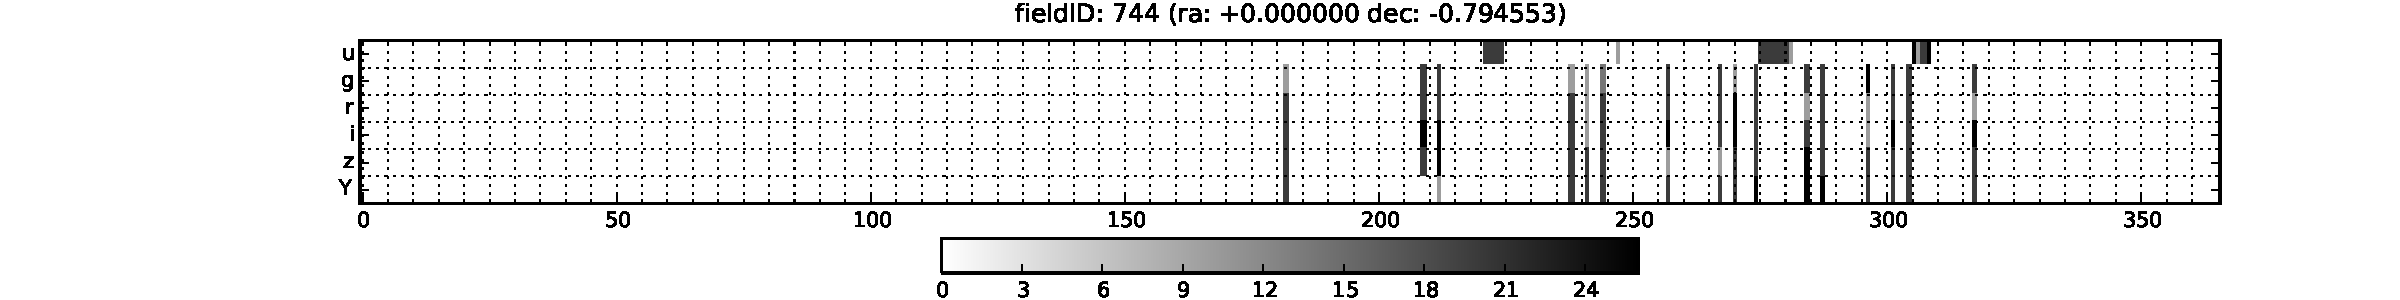
\includegraphics[width=\textwidth]{figs/supernova/fig_firstSeason_0}
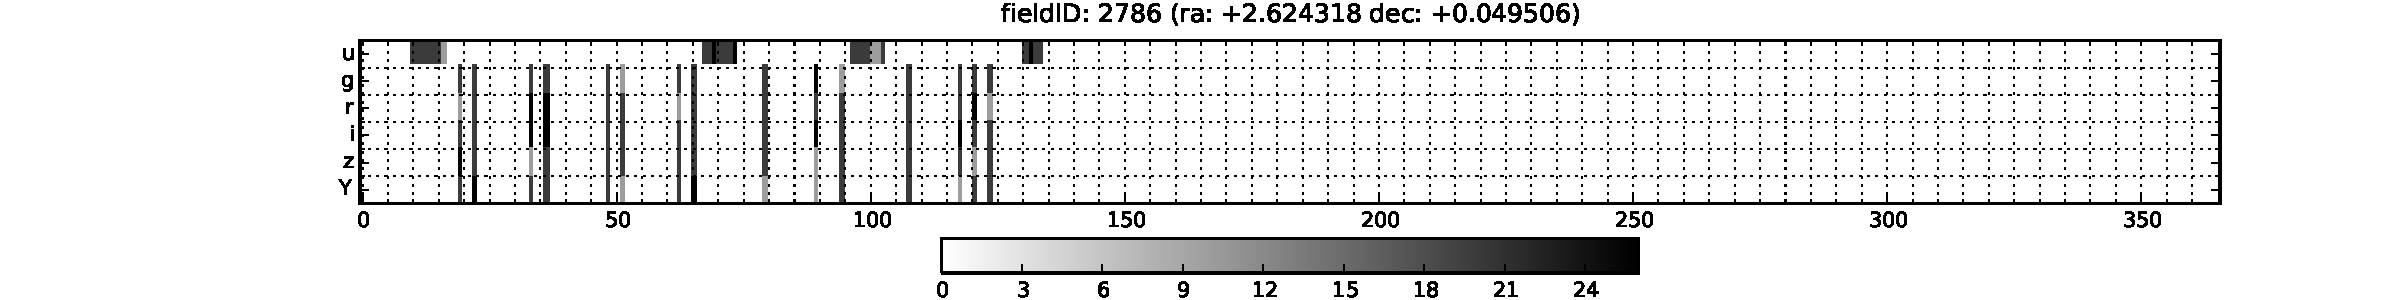
\includegraphics[width=\textwidth]{figs/supernova/fig_firstSeason_1}
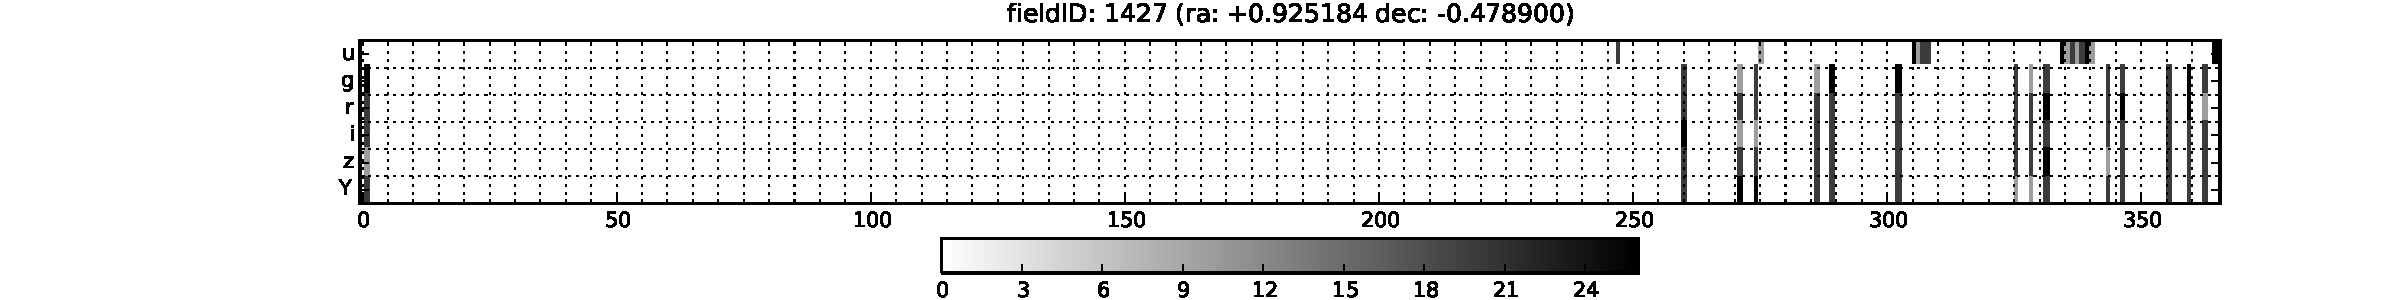
\includegraphics[width=\textwidth]{figs/supernova/fig_firstSeason_2}
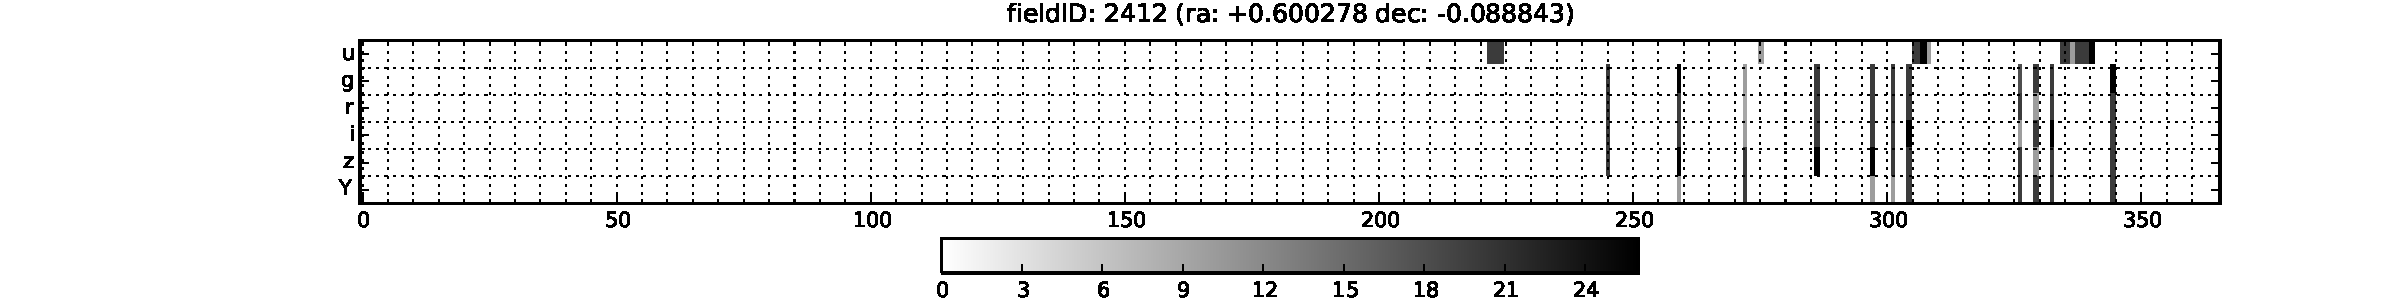
\includegraphics[width=\textwidth]{figs/supernova/fig_firstSeason_3}
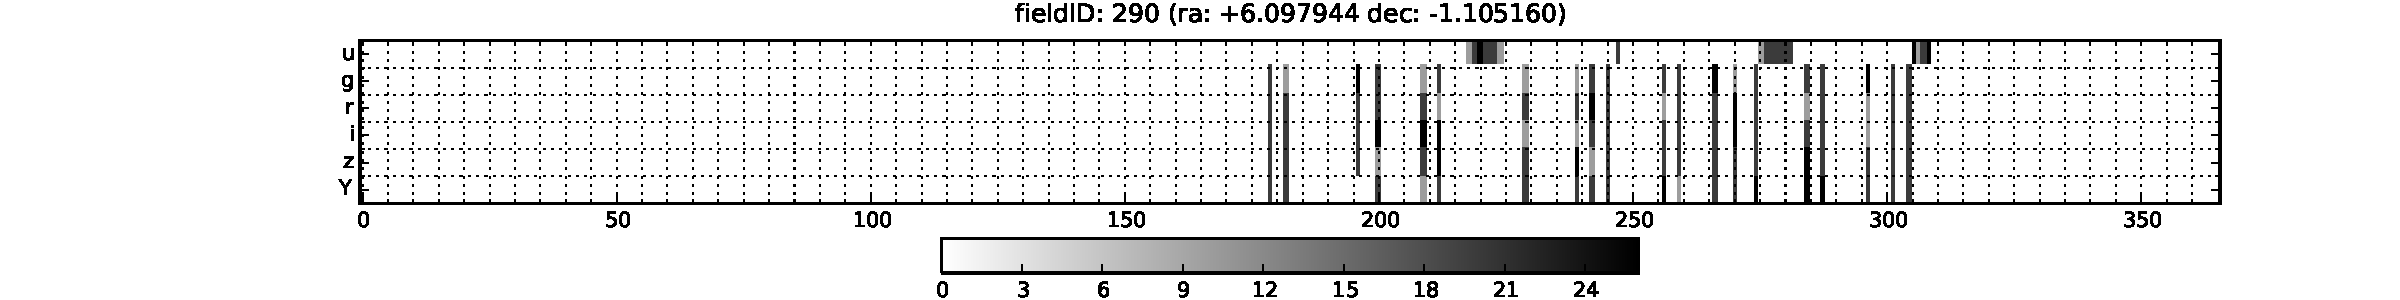
\includegraphics[width=\textwidth]{figs/supernova/fig_firstSeason_4}
\label{fig:opsimSummary}
\caption{Cadence in different filters for a few LSST DDFs in
    the the ouptut of OpSim version Enigma 1189. This ignores issues of chip 
gaps and overlaps between LSST pointings. These issues have been addressed in \citep{CarrollEtal2014} and Awan et.al. (2015, in prep.). We will add these to this analysis.}
\end{figure}



% --------------------------------------------------------------------

\subsection{Discussion}
\label{sec:keyword:discussion}

Discussion: what risks have been identified? What suggestions could be
made to improve this science project's figure of merit, and mitigate
the identified risks?


\begin{itemize}
\item Intrinsic Dispersion, environmental effects, newer analysis methods
\item Follow-up procedures: What is feasible? Where will our training samples for classification and light curve models come from (other experiments, our own 
sub-samples with spectroscopic follow-up?), spectroscopic follow-up of host galaxies. Can hosts be identified?
\item `Systematics': In what ways will the real data not match the assumptions made in analysis. Having a large sample of SN, to understand the astrophysics would be useful for this. 
\end{itemize}


% ====================================================================

\navigationbar


% --------------------------------------------------------------------

\section{Suppressing systematic effects}

Much of cosmology science may be limited by systematic errors rather than photon signal-to-noise.  

\subsection{Target Measurements}

It is expected that even after maximal optimization of camera optics and electronics, that systematic image shape errors will be associated with the orientation of the camera focal plane.  These can be partially reduced by randomization of the orientation of the camera with respect to the sky.  This is represented by the parameter RotSkyPos.  

Similarly, the telescope optics may harbor systematic aberrations, and these also could be mitigated by recording images with varying parallactic angle.  Another relevant parameter, RotTelPos, is indicative of the projected angle of the telescope optics on the sky.  


\subsection{Metrics}

A metric is available for RotSkyPos.  The metric computes, for any selected filter and simulation, a histogram of the distribution of rms values of RotSkyPos computed per field. It also computes basic statistics of these distributions.

\subsection{OpSim Analysis}


\begin{figure}
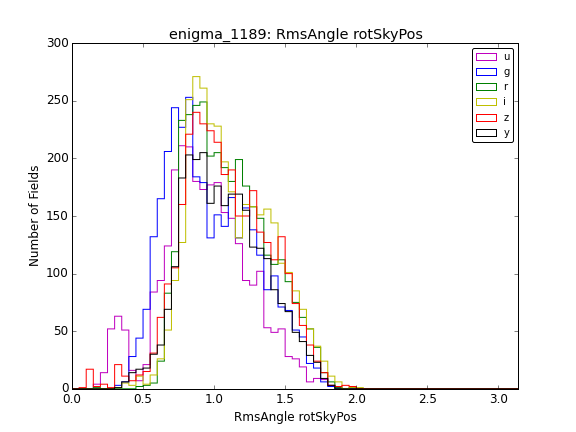
\includegraphics[width=5.0in]{enigma1189RmsAnglerotSkyPosugrizybandallpropsOPSIComboHistogram.png}
\caption{The relative angle of the detector plane with respect to the sky, RotSkyPos, as a histogram showing the number of fields vs. rms of the parameter.}
\label{RotSkyPos}
\end{figure}

The distribution of rms values by filter is shown in Figure \ref{RotSkyPos} for the current candidate baseline simulation, enigma\_1189.  As shown, the rms values cluster around the value 1 radian,  with typical values 1 +- 0.3 radian.  This compares to a completely uniform distribution over the half circle with an rms of 1.14.  

\subsection{Discussion}

The RotSkyPos metric analysis shows that the majority of fields have a good randomization of detector angles projected on the sky.

There are several limitations to this observation.

First, we do not have at present a quantitative requirement for randomization of this parameter.  In future development of weak lensing analysis, a criterion should be developed.

Second, a significant fraction of fields  have median values that are lower or higher than expected for a random distribution, with some far from uniformly distributed.  Regardless of the $per field$ criterion, it is desirable to avoid the incidence of individual discrepant fields.

The recommended criterion for randomization of RotSkyPos is not the behavior of the majority of the fields, but of the minority with the least random behavior.  The number of non-random fields should be minimized.  A recommended metric is the count of fields with median RMS less then 0.8 or greater than 1.5 radians (these values to be reviewed again as additional experience is gained with additional OpSim schedule simulations and weak lensing analysis.)

A similar metric for RotTelPos should be developed. Other observing parameters may benefit from randomization, but are not presently recommended for metric analysis.
